\subsection{The Electron}
Source: \href{https://www.youtube.com/watch?v=rcKilE9CdaA&list=PL8dPuuaLjXtPHzzYuWy6fYEaX9mQQ8oGr&index=6}{The Electron: Crash Course Chemistry \#5}
\\\\
Each orbital describes where the electron is most likely to be found.
\\
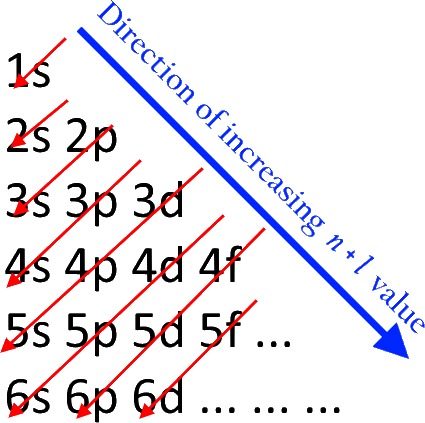
\includegraphics[width=10em]{./includes/chemistry/imgs/Aufbau_Principle.png}

\begin{description}
    \item[Aufbau Principle] Electrons fill orbitals of the lowest energy first.
    \item[Pauli Exclusion Principle] A maximum of two electrons with opposite spin can fit in an orbital.
    \item[Hund's Rule] Electrons will fill all orbitals of a sublevel with one electron before pairing up.
    \item[Octet rule] All tend to have 8 electrons in the outermost shell to become stable.
\end{description}
%
Number of electrons per shell: $2n^2$\\ 
The electron configuration $1\text{s}^2$ means: fist shell, s orbital, 2 electrons\\
The filling sequence is: $1\text{s}^1 \Rightarrow 1\text{s}^2 \Rightarrow 
1\text{s}^2 2\text{s}^1 \Rightarrow 1\text{s}^2 2\text{s}^ 2\Rightarrow 
1\text{s}^2 2\text{s}^2 2\text{p}^1$\\
But: $[\text{Ne}] 3\text{s}^2 3\text{p}^2 \Rightarrow [\text{Ar}] 4\text{s}^1 
\Rightarrow [\text{Ar}] 4\text{s}^2 \Rightarrow [\text{Ar}] 4\text{s}^2 3\text{d}^1$